\documentclass{article}
\usepackage{graphicx}
\usepackage{standalone}
\usepackage{multicol}
\usepackage[parfill]{parskip}

% Used for sequence diagram
\usepackage{pgf-umlsd}
\usepackage{tikz}
\usetikzlibrary{shapes,arrows}

%used for subsubsubsections
\setcounter{tocdepth}{5}
\setcounter{secnumdepth}{5}

\usepackage{changepage}   % for the adjustwidth environment

% for currency
\usepackage{siunitx}

% syntax highlighting
\usepackage{listings} 
\usepackage{color}
\definecolor{lightgray}{rgb}{.9,.9,.9}
\definecolor{darkgray}{rgb}{.4,.4,.4}
\definecolor{purple}{rgb}{0.65, 0.12, 0.82}
\definecolor{codegreen}{rgb}{0,0.6,0}
\definecolor{codegray}{rgb}{0.5,0.5,0.5}
\definecolor{codepurple}{rgb}{0.58,0,0.82}
\definecolor{backcolour}{rgb}{0.95,0.95,0.92}
\lstdefinelanguage{JavaScript}{
  keywords={typeof, new, true, false, catch, function, return, null, catch, switch, var, if, in, while, do, else, case, break},
  keywordstyle=\color{blue}\bfseries,
  ndkeywords={class, export, boolean, throw, implements, import, this},
  ndkeywordstyle=\color{darkgray}\bfseries,
  identifierstyle=\color{black},
  sensitive=false,
  comment=[l]{//},
  morecomment=[s]{/*}{*/},
  commentstyle=\color{purple}\ttfamily,
  stringstyle=\color{red}\ttfamily,
  morestring=[b]',
  morestring=[b]"
}

\lstset{
   language=JavaScript,
   backgroundcolor=\color{lightgray},
   extendedchars=true,
   basicstyle=\footnotesize\ttfamily,
   showstringspaces=false,
   showspaces=false,
   numbers=left,
   numberstyle=\footnotesize,
   numbersep=9pt,
   tabsize=2,
   breaklines=true,
   showtabs=false,
   captionpos=b
}

% Hyperlinks
\usepackage[colorlinks,allcolors=blue]{hyperref}
\usepackage[normalem]{ulem}
\usepackage{xcolor}
\makeatletter
\begingroup
  \catcode`\$=6 %
  \catcode`\#=12 %
  \gdef\href@split$1#$2#$3\\$4{%
    \hyper@@link{$1}{$2}{\uline{$4}}% or \underline
    \endgroup
  }%
\endgroup

\newcommand{\blankpage}{
\newpage
\thispagestyle{empty}
\mbox{}
\newpage
}

%Paths for graphics locations
\graphicspath{ {./}{../../}{../}{TitlePage/}{Abstract/}{Introduction/}{Design/}{Analysis/}{Conclusion/}}
\usepackage{caption}

%Used for bibliography
\usepackage[british]{babel}
\usepackage[%
  autolang=other,
  backend=bibtex      % biber or bibtex
%,style=authoryear    % Alphabeticalsch
 ,style=numeric-comp  % numerical-compressed
 ,sorting=none        % no sorting
 ,sortcites=true      % some other example options ...
 ,block=none
 ,indexing=false
 ,citereset=none
 ,isbn=true
 ,url=true
 ,doi=true            % prints doi
 ,natbib=true         % if you need natbib functions
]{biblatex}
\addbibresource{Bibliography/Bibliography}


\begin{document}

	%Insert title page
	\documentclass{article}
\usepackage{graphicx}


\begin{document}

    \begin{center}
    	%title        
        \Large
        \textbf{The Future of Democracy: Blockchain Voting}
        
        %subtitle
        \vspace{0.2cm}
        \large
        `Ethereum-based voting application proposal'
        
        %university logo
        \vspace{1cm}
        \includegraphics[width=0.9\textwidth]{university}

        \vfill
        
        %team name
        \large
        \textbf{Matthew Flint}
        
        %authors
        \vspace{0.3cm}
        \normalsize
        1247903 - mxf203@bham.ac.uk
        
        %Supervisor
        \vspace{0.3cm}
        \normalsize
        Supervised by Dr. Ian Batten
        
		%description
        \vspace{0.5cm}
		This work was conducted as part of the requirements of the Module 06-26587 `Computer Science Project' of the Computer Science department at the University of Birmingham, UK, and is submitted in accordance with the regulations of the University's code of conduct.
		
		%date at end
		\vspace{0.2cm}
		\today
		
		%remove page number
        \pagenumbering{gobble}
    \end{center}
    \newpage
\end{document}

\blankpage
	
	%Insert the abstract
    \pagenumbering{arabic}
	
	%table of contents
	\cleardoublepage
	\hypersetup{linkcolor=black}
	\tableofcontents
	\newpage

	\documentclass{article}
\usepackage{graphicx}
\usepackage{standalone}
\usepackage{multicol}
\usepackage[parfill]{parskip}


\begin{document}
    \section{Abstract}
   An electronic voting protocol provides end-to-end verifiability if the voter can verify that their vote was correctly counted and any party can verify the results of the election. There have been several proposals outlining potential systems, however these have all been built on top of protocols primarily designed as transaction ledgers. In this paper I propose a voting solution, built on the Ethereum protocol, that uses the properties of smart contracts to enforce strict rules surrounding the ballots of an election. These ballots are both independently and universally verifiable and maintain all of the desirable properties of the blockchain (such as immutability). All of this is achieved without sacrificing voter privacy or ballot integrity. The resulting system shows clear potential for Blockchain technology to become a central part of applications wishing to provide transparency and security in public scenarios.

\end{document}	
	\cleardoublepage

\blankpage

	\documentclass{article}
\usepackage{graphicx}
\usepackage{standalone}
\usepackage{multicol}
\usepackage[parfill]{parskip}


%Used for bibliography
\usepackage[british]{babel}
\usepackage[%
  autolang=other,
  backend=bibtex      % biber or bibtex
%,style=authoryear    % Alphabeticalsch
 ,style=numeric-comp  % numerical-compressed
 ,sorting=none        % no sorting
 ,sortcites=true      % some other example options ...
 ,block=none
 ,indexing=false
 ,citereset=none
 ,isbn=true
 ,url=true
 ,doi=true            % prints doi
 ,natbib=true         % if you need natbib functions
]{biblatex}
\addbibresource{../Bibliography/Bibliography}

\begin{document}
    \section{Introduction}
Existing electronic voting systems all suffer from a serious design flaw; they are centralised by design, meaning there is a single supplier that controls the code base, the database and the system outputs while also supplying the monitoring tools to verify the result \citep{3_noizat_2016}. The lack of an independently verifiable system means that, once voters mark their ballot choice, they must place their trust in the organization that their vote is recorded and counted as intended. The lack of an independently verifiable output makes it difficult for these centralized systems to acquire the trustworthiness required by voters, which potentially limits voter participation, or cast doubt upon the published outcome of an election.

Despite the digitalisation of many aspects of modern life, elections are still being largely conducted offline, on paper \citep{43_ernest_2014}, although the use of Electronic Voting Machines has been steadily growing over recent years. Paper ballots are still the traditional tool for voting and are typically marked by a human (voter) and then tallied by a machine. While costing less than most electronic systems to run, they rely on physical security and trust in polling stations to not manipulate and properly handle them \citep{44_wyndham_chen_das_2016}. Postal votes also utilize paper ballots and are used to allow voters to not have to physically attend a location in order to vote. These also suffer from the same flaws as traditional paper ballots while increasing the opportunities for attack during their passage through the postage system.

Voting systems comprise of five main components:
\begin{enumerate}
	\item A registration service for verifying and registering legitimate voters.
	\item Voter authentication stations with the task of determining a voters authorization to vote based on the completed work of the registration service.
	\item Voting stations where the voter makes choices on a ballot.
	\item A device called the ballot box where the ballot is collected.
	\item A tallying service that counts the votes and announces the results.
\end{enumerate}
Of the components listed above, only \verb|(2)|, \verb|(3)| and \verb|(4)| are used during an election, with \verb|(1)| being being required for an election to take place and \verb|(5)| happening post election \citep{48_safevote_2001}.

Current Electronic Voting (E-Voting) takes two forms; using a machine in a polling station, rather than a ballot paper and pencil, or casting a vote over the Internet. The former tends to refer to a Direct Recording Electronic system which typically displays ballot options on a screen that can be activated by the voter and then records that voting data in memory components to be processed later. However, as with many electronics, there is the inherent problem of the ability to modify software and potentially insert malicious code \citep{44_wyndham_chen_das_2016}. This has been an issue raised over several recent elections and a study from 2015 concluded that 43 American states would be using Electronic Voting Machines that are at least 10 years old during the last presidential election \citep{45_holmes_2016}. Voting over the Internet, while having to deal with issues such as privacy, fraud, voting under duress, and corruption, does nothing to improve a voter's trust. The voter must still assume that once they have cast their vote it will be recorded and counted honestly.

In order for our proposed E-Voting system to be a tangible challenger to more traditional voting methods, it must be able to provide the current systems' services, at least at the same level but preferably with improvements, while also providing substantial benefits. There are several standard requirements that a voting system should adhere to, each holding equal weight: security, functionality, privacy, usability, and accessibility \citep{46_voting_system_standards_testing_and_certification_2016}. A ``secure'' voting system means one that cannot be tampered with or manipulated in any way, ensuring that votes are accurately recorded as cast. It also ensures that additional votes cannot be cast after the polls have closed or tampered with at any stage of the process. System functionality can be broad but should include; The correct registering and recording of all votes cast, permitting a voter to vote for any candidate they have the right to vote for, allowing only eligible registered voters to vote and only allowing each voter to vote once. Voters have the right to a secret ballot and to cast their vote in private \citep{46_voting_system_standards_testing_and_certification_2016}. This is essential to protect voters from being coerced or bribed into voting a certain way, this means that our system should not provide a receipt or any way for another person to determine the contents of a voter's ballot. On top of this the system should be easy for voters to use, meaning it's as intuitive as possible, and maintain universal vote access. It should avoid introducing bias by selecting platforms that are less available to some groups than to others as the choice of the language, ballot format, or devices may seem innocuous, but it may actually prevent small factions of the voters to cast their vote \citep{47_petride_2016}.

Whilst maintaining these essential foundations already provided in traditional voting systems, there are several improvements and additions which I intend to explore. The first benefit in using a blockchain to log votes is in its decentralised nature. This means there is less need for trust to be placed in a centralised organization where votes are hidden behind closed doors. It also has the benefit of being significantly harder to tamper with as, once a transaction has been verified, an attacker would need to possess at least 51\% of the computing power of the network to attempt to forge transactions. Any attempts to otherwise use a forged block will be noticed by the rest of the network and ignored. This decentralized system also brings in more transparency as anyone can view, transactions in the blockchain leading to higher levels of trust in the elections outcome. This is further strengthened by the independent verifiability which could be performed by anyone, therefore removing the need to trust the election organizers' declaration of the outcome. Once a transaction (vote) has been confirmed in the blockchain (and has further blocks built upon it) this vote for a candidate becomes immutable, meaning that the entire outcome of an election will be stored indefinitely, and is able to be accessed at any time in the future.

Verifiability properties of electronic voting are divided in two categories. ``Individual verifiability'', which involves auditing the processes of vote creation and vote storage by the voter; and ``Universal verifiability'', which ensures that only votes from eligible voters are stored in the ballot box and that all stored votes are properly tallied, which can be performed by anyone \citep{49_escala_guasch_herranz_morillo_2015}. Systems providing both types of verifiability are known as ``end-to-end verifiable systems''.

One of the individually verifiable properties is cast-as-intended verification, which is focused on the audit of the vote creation process. Another property is recorded-as-cast verification, aimed at auditing the correct reception and storage of the vote in a remote voting server \citep{49_escala_guasch_herranz_morillo_2015}.


In this paper I outline the design of an ``end-to-end verifiable system'' built on the Ethereum Blockchain. In this system, a voter can register an Ethereum address which is then added to a list of \textit{allowed addresses} inside a smart contract. Upon the ballot commencing, the voter will be able to modify the allocation of their vote inside this contract up to the point of the ballot ending. Due to the programmable nature of Ethereum contracts we can be sure that; no votes can be modified after the ballots end date, only the voter in control of the Ethereum address can change the vote associated with that address and only Ethereum addresses pre-registered to the contract are able to vote. Anyone can verify the number of votes for a candidate by querying the contract, and as they can be assured that only those addresses added to the contract are able to vote, we can be sure of the validity of each of these votes. 

%\printbibliography

\end{document}	
	\cleardoublepage

\blankpage

	\documentclass{article}
\usepackage{graphicx}
\usepackage{standalone}
\usepackage{multicol}
\usepackage[parfill]{parskip}


%Used for bibliography
\usepackage[british]{babel}
\usepackage[%
  autolang=other,
  backend=bibtex      % biber or bibtex
%,style=authoryear    % Alphabeticalsch
 ,style=numeric-comp  % numerical-compressed
 ,sorting=none        % no sorting
 ,sortcites=true      % some other example options ...
 ,block=none
 ,indexing=false
 ,citereset=none
 ,isbn=true
 ,url=true
 ,doi=true            % prints doi
 ,natbib=true         % if you need natbib functions
]{biblatex}
\addbibresource{../Bibliography/Bibliography}

\begin{document}
    \section{Background}
    \subsection{Evaluation of Previous Research}

There has been some research conducted in this area already and several protocols for blockchain based voting have been proposed. \textit{Pierre Noizat} proposes a system \citep{3_noizat_2016} where each candidate provides a unique public key, KeyC, to each individual voter along with a singular bitcoin address, AddressC, which the final sum of the voting transactions will be sent to. Each voter is also assigned an individual public key, KeyA, by the election organizers and, either they generate a key pair themselves (this could be done by the voting software for better usability), KeyB, or be assigned the KeyB by the organization. From these three public keys, the voter can generate a \verb|2-of-3| multi signature address which represents the vote of B in favour of C. This address is then funded with a bitcoin micropayment (around the price of a postage stamp), either by the voter or organisation, and this is the voters confirmation of their vote. After a few hours this ballot is securely logged on the blockchain and, as the multisignature address was funded, a voter can check that this address is represented in the blockchain and that their vote was registered. It should be noted that there is no way to guess neither the voter (B) nor the candidate (C) from a multisignature address without knowing all three public keys (KeyA, KeyB, and KeyC) and knowing to whom they belong. Once the election is concluded the organization is able to, via the \verb|2-of-3| multi signature address, spend the coins the voter gave to the candidate to fund the address of the candidate, AddressC. This provides an unequivocal link between the vote and the candidate which can be seen and validated by anyone.

While the proposed method does provide a valuable alternative to current proprietary electronic voting systems and has the benefits of; protecting the secrecy of the ballots, allowing free, independent audits of the results and minimizing the trust level required from the organizers \citep{3_noizat_2016}. It does come with several drawbacks; the independent validation of votes before the organization funds a candidate's public address, AddressC, can only be done by the voting individual on their ballot choice. The protocols dependence on the Bitcoin blockchain could pose problems with subsequent elections as there is no definitive boundary between one election and the next. The currency units, although in very small denominations, could be transferred out of the election to private addresses for an individual's gain (though even if 100\% of the vote currency was lost, the cost of an election would likely be less than if done using current methods).

Another proposal is that of Universal Cast-as-Intended Verifiability \citep{49_escala_guasch_herranz_morillo_2015} which allows any party (not only the voter) to publicly verify that an encrypted cast vote really matches the selection of a voter. Their proposal allows a voter who's eligible to vote to register with a registrar, who then generates a pair of public-secret values for each voting option in the election. These secret values are sent to the voter, while the public ones are published, linked to the voting options they are related to. During the voting phase, the voter provides her selected voting options and a subset of the secret values she received during registration to the voting device. The voting device then encrypts the voters selections and creates a non interactive zero-knowledge proof, which will be valid only in the case that the voting device encrypted what the voter selected. Due to the zero-knowledge property of the proofs, they can be publicly verified while maintaining the voters privacy.

While this may seem like a vastly superior proposal on the surface, the additional complexity of the underlying system, that is the inclusion of zero-knowledge proofs, should not be underestimated. Furthermore, zero-knowledge protocols, despite being proposed in the late 1970s, are still in their relative infancy when compared to Blockchain technology (e.g. zCash whitepaper \citep{50_ben-sasson_chiesa_garman_green_miers_tromer_virza_2014}, 2014) and therefore have not been through the same level of scrutiny nor do they have the same level of development or adoption. The protocol also requires the voter to supply a secret value for each of the voting options they did not choose which, may require considerable effort if the ballot is large enough, and is counter intuitive to what would usually be expected to cast a vote.

\clearpage
\subsection{Ethereum}
\subsubsection{What is Ethereum}
In summary, Ethereum is an open software platform based on blockchain technology that enables developers to build and deploy decentralized applications. The block chain is a decentralized network of computers who, at the most basic level, all maintain a ledger in consensus with each other. One block is added at a time, each block contains a mathematical proof that verifies it's addition to the chain and the transactions within are protected by a strong cryptography.
 
Ethereum is poised to become the next greatest innovation based on block chain technology. So is Ethereum similar to Bitcoin? It does have similarities, but not really. Like Bitcoin, Ethereum is a distributed public blockchain network, however there are some significant technical differences between the two. The most important distinction to note is that Bitcoin and Ethereum differ substantially in purpose and capability. Bitcoin offers one particular application of blockchain technology, a peer to peer electronic cash system that enables online payments. While the bitcoin blockchain is used to track ownership of digital currency (bitcoins), the Ethereum blockchain focuses on running the programming code of decentralized application \citep{55_what_is_ethereum_a_step-by-step_beginners_guide_2017}.

Ethereum enables developers to build and deploy decentralized applications. A decentralized application or `Dapp' serves some particular purpose to its users, for example Bitcoin, is a Dapp that provides its users with a peer to peer payment system. Because decentralized applications are made up of code that runs on a blockchain network, they are not controlled by any individual or central entity. Running these Dapps on a decentralized platform, the blockchain, means they benefit from all of its properties \citep{54_ethereum_explained_2017}:

\begin{itemize}
	\item Immutability, a third party cannot make any changes to data.

	\item Corruption and tamper proofing, as apps are based on a network formed around the principle of consensus, making censorship impossible.

	\item No central point of failure, as Dapps can be run on every node in the network.

	\item Secured using cryptography, applications are well protected against hacking attacks and fraudulent activities.

	\item Zero downtime, Dapps never go down and can never be switched off.

\end{itemize}

\clearpage
\subsubsection{Ethereum Blockchain}
The concept of the blockchain was originally outlined in a white paper \citep{12_nakamoto_2008} authored under the pseudonym Satoshi Nakamoto in November of 2008 and was quickly followed by an open source release of the Bitcoin proof-of-concept source code in January 2009 \citep{13_nakamoto_2009}. This is the distributed ledger which underpins the entirety of the Bitcoin and Ethereum systems. A distributed ledger is a consensus of replicated, shared, and synchronized digital data geographically spread across multiple sites, countries, and/or institutions \citep{24_distributed_ledgers_and_blockchain_technology_2016}. This ledger is stored locally on every node in the network which is running the full version of the blockchain software \citep{14_bitcoin_2009} and records every transaction sent and confirmed on the network (the current size of the Ethereum Blockchain is around 21GB, March 2017\citep{25_blockchain_size_2016}). This complete history, coupled with the fact that it is an open network, means that anyone can see what is happening in the network, not just now but during all periods in the past. This is extremely powerful as it allows an individual to fully audit the entire contents of the Blockchain without relying on external parties. This process is, in fact, what happens when you first download the full version of many blockchain reliant software \citep{20_developer_guide_bitcoin_2016}.

While the Ethereum Blockchain is not the only most mature distributed ledger in existence, it does have several years of being a publicly proven method to achieve distributed consensus and does this via the `proof-of-work mining' process \citep{24_distributed_ledgers_and_blockchain_technology_2016}. This is how new information gets added to the blockchain, by nodes in the network running a special `mining' variant of the Ethereum software which uses considerable computing resources to win the right to add another block to the Blockchain, which is accompanied by a reward for the winning user. The concept of `proof-of-work' is a method of ensuring that the information being added to the Blockchain was difficult (in terms of cost and time) to be made, though is easy for others to validate that the requirements were met \citep{26_blockchain_mining_-_distributed_ledgers_and_blockchain_technology_2016}. This means that the expenditure of computing power serves to secure the integrity of the Blockchain, while the miners themselves verify through public-private key cryptography the validity of each transaction they include in a block.

Blocks are chained together making it impossible to modify transactions included in any one block without modifying all following blocks; as a result, the cost to modify a particular block increases with every new block added to the block chain, magnifying the effect of the proof of work \citep{20_developer_guide_bitcoin_2016}\citep{38_proof_of_work_-_masterpage_2016}. This is why, although a transaction is deemed clear upon its inclusion in a block on the Blockchain, best practices dictate that a user considers a transaction confirmed after its inclusion in a block and the addition of five subsequent blocks to the Blockchain \citep{27_confirmation_-_bitcoin_wiki_2016}.

The difficulty of the proof-of-work mining needs to be controlled, so that an average mining time of around 12 seconds per block is maintained. This time is somewhat arbitrary but is an attempt to find a balance between accepting transactions quickly and minimizing instability and waste in the network, as, while a new block is being distributed other miners will be working on an obsolete problem. As more miners join the network the block creation rate will increase due to the greater collective computational power. Therefore, every 2,016 blocks the difficulty of the mathematical challenge is recalculated so that the average mining time returns to normal \citep{20_developer_guide_bitcoin_2016}\citep{26_blockchain_mining_-_distributed_ledgers_and_blockchain_technology_2016}.

Despite the media often suggesting that bitcoin (and the Blockchain technology behind it) is an anonymous payment system, the Blockchain is in fact a transparent record of all user transactions on the network. Blockchain transactions are in fact pseudonymous, and your transactions in the network are like writing under a pseudonym. If an author's identity is ever linked to their pseudonym then everything written under that pseudonym will be revealed \citep{28_anonymity_2016}. This is particularly poignant when considering the Blockchain as every transaction is stored forever, therefore a compromised address could lead to all transactions being linked to a person. There are however ways to reduce the amount of statistical analysis which can be done on transactions that a person is a part of which help to achieve reasonable anonymity \citep{76_chan_liu_xeu_2013}.

\subsubsection{Mining and Ether}
Ether is the fuel of the Ethereum system. It is the currency of the Ethereum network with which the payment of computation is achieved. Ethereum, like all blockchain technologies, uses an incentive-driven model of security where transaction consensus is based on a ``proof-of-work'' criterion of a given difficulty.

The block chain on which the Ethereum executes certain environment is known as the Ethereum Virtual Machine (EVM) \citep{54_ethereum_explained_2017}. Each participating node within the network runs the EVM and performs the proof of work algorithm called Ethash which involves finding a nonce input to the algorithm so that the result is below a certain threshold (depending on the difficulty) \citep{57_introduction_ethereum_frontier_guide_2017}. There is no better strategy to find such a nonce than enumerating the possibilities while verification of a solution is trivial and cheap. If outputs have a uniform distribution, then we can guarantee that on average the time needed to find a nonce depends on the difficulty threshold, making it possible to control the time of finding a new block just by manipulating difficulty \citep{57_introduction_ethereum_frontier_guide_2017}.

This is the process of how transactions are validated, new transactions are forwarded around the network and placed into a pool of unconfirmed transactions. These are not considered `accepted' yet but are available for all to see almost instantaneously. Miners draw from this pool to create a candidate next set of transactions to be officially accepted which will form the next block. The full text of all of these candidate transactions, along with the hash of the previous block and a nonce, are input into the the hash function (Ethash) and miners will try different values for the nonce until the resulting hash is below a certain value. Because it's a cryptographic hash, there's no way to find a nonce that satisfies the output hashes condition other than attempting to guess \citep{20_developer_guide_bitcoin_2016}. At this point, all of the miners are in a competition to find the hash first, each with a potentially different set of transactions to confirm. Once a miner succeeds they announce their solution to the rest of the network, their block becomes the next block in the Blockchain, and the transactions therein become confirmed. This strategy means that one miner will choose the next set of confirmed transactions, but the hash function effectively makes the miner a random one. All other mines then validate this new block, and the transactions held within, and can choose to accept it and start work on the next block. As the new block contains the hash of the previous block, this forms a chain of confirmed blocks securing the order of the transactions held within.

Occasionally, two miners may find a solution to the problem at the same time creating two potential next blocks in the chain. When miners produce simultaneous blocks at the end of the block chain, each node individually chooses which block to accept, this is usually the first block they see. Eventually another miner finds the solution to another block which attaches to only one of the competing blocks. This makes that side of the fork stronger and, as the general consensus is to use the strongest chain, other nodes will switch to this longer Blockchain \citep{20_developer_guide_bitcoin_2016}. While this is statistically unlikely to happen, it is even more unlikely for the subsequent blocks to be solved at the same time, meaning that one fork will grow quicker than the other and the fork will resolve itself quickly. Transactions that were in the fork that wasn't chosen are not lost and are placed back into the unconfirmed transactions pool \citep{4_driscoll_2016}. The fact that the end of the chain can be forked and rearranged means you shouldn't trust transactions at the end of the chain as much as ones further back. In Ethereum, a transaction is not considered confirmed until it is part of a block in the longest fork, and at least five blocks follow it. In this case we say that the transaction has ``5 confirmations''. This gives the network time to come to an agreed-upon the ordering of the blocks \citep{35_nielsen_2013}.

The successful miner of a block receives a reward for the `winning' block, consisting of exactly 5.0 Ether along with all of the gas expended within the block, that is, all the gas consumed by the execution of all the transactions in the block. Over time, it's expected the gas reward will dwarf the block reward and become the main incentive for miners to continue working \citep{57_introduction_ethereum_frontier_guide_2017}.

\subsubsection{Transaction Costs and Gas}
Ethereum does have a small transaction fee, just like Bitcoin, where users pay a relatively small amount to the executor of your transaction. The sender has to pay the fees at each and every step of the activated program, this includes the memory, storage and computation \citep{54_ethereum_explained_2017}. The size of the fee paid is equivalent to the complexity of the transaction, i.e. the more complex the commands you wish to execute, the more gas (and Ether) you have to pay. For example if ``Alice'' wants to send ``Bob'' 1 Ether unit, there would be a total cost of 1.00001 Ether to be paid by Alice. However if A wanted to deploy a contract or run a contract function, there would be more lines of code executable, therefore more energy consumption placed on the distributed Ether network and she would have to pay more than the 1 Gas done in the first transaction \citep{56_ethereum_2017}. Some computational steps cost more than others, either because they are more computationally expensive or because they increase the amount of data that has to be stored in the state. 

Gas is the internal pricing for running a transaction or contract in Ethereum. The gas system is not very different from the use of kilowatts in measuring electricity except that the originator of the transaction sets the price of gas, to which the miner can or not accept \citep{56_ethereum_2017}. Ether and Gas are inversely related say for instance if the Ether price increases, than Gas price should decrease to maintain the concept of real cost \citep{54_ethereum_explained_2017}. There is also a blocksize limit, so the more space your transaction takes up the more you have to pay to get it validated. With Bitcoin, miners prioritise transaction with the highest mining fees. The same is true of Ethereum where miners are free to ignore transactions whose gas price limit is too low. 

The reason for the inclusion of a gas price per transaction or contract is to deal with the Turing Complete nature of Ethereum and its EVM essentially to guarantee that code running in the network will terminate. So for example, 0.00001 Ether or 1 Gas can execute a line of code or some command. If there is not enough Ether in the account to perform the transaction or message then it is considered invalid. This aims to stop denial of service attacks from infinite loops, encourage efficiency in the code and make any potential attacker pay for the resources they use (whether that be bandwidth, CPU cycles or storage) \citep{56_ethereum_2017}.

\subsubsection{Smart Contracts}
\label{sec:SmartContracts}
Smart contracts are the key element of Ethereum. In them, any algorithm can be encoded, they can carry arbitrary state and can perform any arbitrary computations even being able to call other smart contracts. This gives the scripting capabilities of Ethereum tremendous flexibility \citep{59_peyrott_senanayaka_2017}. When run a smart contract becomes like a self-operating computer program that automatically executes when specific conditions are met and because they run on the blockchain, they run exactly as programmed without any possibility of censorship, downtime, fraud or third party interference. While all blockchains have the ability to process code, most are severely limited. Ethereum is different in this respect as rather than giving a set of limited operations, Ethereum allows developers to create whatever operations they want allowing developers to build thousands of different applications that go far beyond anything seen previously \citep{55_what_is_ethereum_a_step-by-step_beginners_guide_2017}.

The Ethereum Virtual Machine is where smart contracts are run. It provides a more expressive and complete language than bitcoin for scripting and is Turing Complete. A good metaphor is that the EVM is a distributed global computer where all smart contracts are executed \citep{58_the_hitchhikers_guide_to_smart_contracts_in_ethereum_2017}. There are several higher level languages used to program smart contracts, but Solidity is the most mature and widly adopted. Its syntax is similar to that of JavaScript, its statically typed, supports inheritance, libraries and complex user-defined types among other features.

Smart contracts are run by each node as part of the block creation process and, just like in Bitcoin, this is the moment where transactions actually take place. An important part of how smart contracts work in Ethereum is that they have their own unique address in the blockchain. In other words, contract code is not carried inside each transaction that makes use of it. Instead contracts are ``deployed'' to the blockchain in a special transaction that assigns an address to a contract. This transaction can also run code at the moment of creation. After this initial transaction, the contract becomes forever a part of the blockchain and its address never changes. Whenever a node wants to call any of the methods defined by the contract, it can send a message to the address of the contract, specifying data as input and the method that must be called. The contract will then run as part of the creation of newer blocks up (subject to the gas limit or completion) and can return a value or store data \citep{59_peyrott_senanayaka_2017}.

\end{document}	
	\cleardoublepage

	\documentclass{article}
\usepackage{graphicx}
\usepackage{standalone}
\usepackage{multicol}
\usepackage[parfill]{parskip}

% Used for sequence diagram
\usepackage{pgf-umlsd}
\usepackage{tikz}
\usetikzlibrary{shapes,arrows}

% Hyperlinks
\usepackage[colorlinks,allcolors=blue]{hyperref}
\usepackage[normalem]{ulem}
\usepackage{xcolor}
\makeatletter
\begingroup
  \catcode`\$=6 %
  \catcode`\#=12 %
  \gdef\href@split$1#$2#$3\\$4{%
    \hyper@@link{$1}{$2}{\uline{$4}}% or \underline
    \endgroup
  }%
\endgroup
%Used for bibliography
\usepackage[british]{babel}
\usepackage[%
  autolang=other,
  backend=bibtex      % biber or bibtex
%,style=authoryear    % Alphabeticalsch
 ,style=numeric-comp  % numerical-compressed
 ,sorting=none        % no sorting
 ,sortcites=true      % some other example options ...
 ,block=none
 ,indexing=false
 ,citereset=none
 ,isbn=true
 ,url=true
 ,doi=true            % prints doi
 ,natbib=true         % if you need natbib functions
]{biblatex}
\addbibresource{../Bibliography/Bibliography}

\begin{document}
    \section{Design}
    
    \subsection{Overview}
    
In this paper, I present an ``end-to-end verifiable system'' built on the Ethereum Blockchain, i.e., a system where a voter can be assured their vote has been fairly counted, only eligible voters are allowed to vote and the tallied results of the election are publicly verifiable.

Although this system has been designed and developed with the idea of a national general election in mind, the protocols and ideas involved could be applied to smaller scale ballots which wish to provide transparency in their audit. Although we wish to minimize trust in a central authority, due to the nature of these type of elections (where there needs to be some degree of voter eligibility verification), we cannot fully decentralize this system as we need to only allow those eligible the rights to vote. Despite needing to verify an individual we still need to ensure that their votes are publicly anonymous, especially given the public transactions underpinning the blockchain concept while providing the ability for an individual to verify that their vote was correctly counted.

I do not see this system as a direct ``replace all'' for national election voting. I believe there will still be a need for traditional voting implementations in certain situations; for example, maintaining postal vote for the elderly who may not have the technical capability or equipment for online voting. However I do think that this could be phased in along side traditional voting, eventually replacing the pre-existing e-voting systems and ultimately becoming the main way for the majority of people to choose their government. 

The designed schema for this protocol is the following:
\begin{enumerate}

\item Ballot creation:
	\begin{itemize}
		\item The available ballots in the election are designed and decided upon.
		\item A smart contract is created and pushed to the blockchain for each ballot containing all of the voting options.
	\end{itemize}

\item Pre-election voter verification:
	\begin{itemize}
		\item Voter registers with an external voter registrar after providing a valid ID (this could be accomplished using pre-existing government electoral registration protocols).
		\item This external registrar generates a \textit{user\_id} and \textit{nonce} which can be used by the voter to log in to the system.
		\item This \textit{user\_id} is then tied to any ballots the voter is eligible for.
	\end{itemize}
	
\item Voter registration:
	\begin{itemize}
		\item The voter logs into the system using the received \textit{user\_id} and nonce upon which time they are immediately required to change their login credentials.
		\item The voter can then register to vote through the online system for each of the ballots they are eligible for.
		\item A unique Ethereum address, \textit{voter\_address}, is generated and validated (while not being linked to the \textit{user\_id})
		\item The \textit{user\_address} is added to the ballots smart contract which entitles this address to vote in that ballot.
		\item The address is funded with enough Ether for the voter to cast their vote.
	\end{itemize}

\item Voting:
	\begin{itemize}
		\item When the voter decides to cast their vote they are presented with an interface mirroring the options in the ballot smart contract.
		\item Upon the voter selecting their options the contract is funded with the voters selected options.
		\item At this point the voters choice is immutably entered into the blockchain and the tally is verifiable by all.
	\end{itemize}

\item Election result:
	\begin{itemize}
		\item Once the election is over, due to the nature of the smart contract design, no more votes can be added for any candidate.
		\item The tally for each candidate is publicly verifiable by anyone along with all of the funded transactions casting votes.
	\end{itemize}

\end{enumerate}

\cleardoublepage    
\subsection{Docker}
Over the past few years, container technology has become increasingly promising as a means to seamlessly make software available across a wider range of platforms \& allow developers to worry less about the eventual runtime environment (as this can be standardized). Docker containers provide a way to ``wrap up a piece of software in a complete filesystem that contains everything it needs to run'' {\LARGE [51]}.

There are several benefits to the use of Docker containers; This could substantially reduce the effort required to create and validate a new software releases, since docker containers create their own dedicated environment, testing on one OS means that the application will run the same on any OS capable of running Docker. In addition, docker containers provide a quick and easy way to install and use a software release, for our application this could mean faster patches if needed as you would simply need to swap out the docker image being used. Other benefits include faster bootup of containers (compared to just virtualization), closer development to production parity, immutable infrastructure and improved scaling (on a per-container basis) {\Large [52]}. There is also a security argument to be made for using containers, as they offer a degree of isolation for each enclosed application and only expose those services which you decide. The previous point about patching also add to security, as legacy applications often forgo patches in sensitive environments due to the possibility of breakages. When using containers, changes can be fully tested in the container which can then be swapped into the production environment {\LARGE [53]}.

All of my development for this project was conducted inside of Docker containers. I decided on this because there are very distinct separations between the applications which make up my system (this is described in section {\Large LINK TO SECTION}), so running each one inside a docker container seemed the logical thing to do. It also meant that I could control the startup of the system as a whole \& expose (between containers) only those services necessary to communicate.

\cleardoublepage
\subsection{Ethereum}
\subsubsection{What is Ethereum}
In summary, Ethereum is an open software platform based on blockchain technology that enables developers to build and deploy decentralized applications. The block chain is a decentralized network of computers who, at the most basic level, all maintain a ledger in consensus with each other. One block is added at a time, each block contains a mathematical proof that verifies it's addition to the chain and the transactions within are protected by a strong cryptography.
 
Ethereum is poised to become the next greatest innovation based on block chain technology so is Ethereum similar to Bitcoin? The answer is sort of, but not really. Like Bitcoin, Ethereum is a distributed public blockchain network, however there are some significant technical differences between the two. The most important distinction to note is that Bitcoin and Ethereum differ substantially in purpose and capability. Bitcoin offers one particular application of blockchain technology, a peer to peer electronic cash system that enables online payments. While the bitcoin blockchain is used to track ownership of digital currency (bitcoins), the Ethereum blockchain focuses on running the programming code of decentralized application {\Large [55]}.

Ethereum enables developers to build and deploy decentralized applications. A decentralized application or Dapp serves some particular purpose to its users, for example Bitcoin, is a Dapp that provides its users with a peer to peer payment system. Because decentralized applications are made up of code that runs on a blockchain network, they are not controlled by any individual or central entity. Running these Dapps on a decentralized Platform, the blockchain, they benefit from all of its properties {\Large [54]}:

\begin{itemize}
	\item Immutability, a third party cannot make any changes to data.

	\item Corruption \& tamper proof as apps are based on a network formed around the principle of consensus, making censorship impossible.

	\item No central point of failure, as Dapps can be run on every node in the network.

	\item Secured using cryptography, applications are well protected against hacking attacks and fraudulent activities.

	\item Zero downtime, Dapps never go down and can never be switched off.

\end{itemize}

\cleardoublepage
\subsubsection{Ethereum Blockchain}
The concept of the blockchain was originally outlined in a white paper \citep{12_nakamoto_2008} authored under the pseudonym Satoshi Nakamoto in November of 2008 and was quickly followed by an open source release of the Bitcoin proof-of-concept source code in January 2009 \citep{13_nakamoto_2009}. This is the distributed ledger which underpins the entirety of the Bitcoin and Ethereum systems. A distributed ledger is a consensus of replicated, shared, and synchronized digital data geographically spread across multiple sites, countries, and/or institutions \citep{24_distributed_ledgers_and_blockchain_technology_2016}. This ledger is stored locally on every node in the network which is running the full version of the blockchain software \citep{14_bitcoin_2009} and records every transaction sent and confirmed on the network (the current size of the Ethereum Blockchain is around 21GB, March 2017\citep{25_blockchain_size_2016}). This complete history, coupled with the fact that it is an open network means that anyone can see what is happening in the network, not just now but during all periods in the past. This is extremely powerful as it allows an individual to fully audit the entire contents of the Blockchain without relying on external parties. This process is, in fact, what happens when you first download the full version of many blockchain reliant software \citep{20_developer_guide_bitcoin_2016}.

While the Ethereum Blockchain is not the only most mature distributed ledger in existence, it does have several years of being a publicly proven method to achieve distributed consensus and does this via the `proof-of-work mining' process \citep{24_distributed_ledgers_and_blockchain_technology_2016}. This is how new information gets added to the blockchain, by nodes in the network running a special `mining' variant of the Ethereum software which uses considerable computing resources to win the right to add another block to the Blockchain which is accompanied by a reward for the winning user. The concept of `proof-of-work' is a method of ensuring that the information being added to the Blockchain was difficult (in terms of cost and time) to be made, though is easy for others to validate that the requirements were met \citep{26_blockchain_mining_-_distributed_ledgers_and_blockchain_technology_2016}. This means that the expenditure of computing power serves to secure the integrity of the Blockchain, while the miners themselves verify through public-private key cryptography the validity of each transaction they include in a block.

Blocks are chained together making it impossible to modify transactions included in any one block without modifying all following blocks; as a result, the cost to modify a particular block increases with every new block added to the block chain, magnifying the effect of the proof of work \citep{20_developer_guide_bitcoin_2016}\citep{38_proof_of_work_-_masterpage_2016}. This is why, although a transaction is deemed clear upon its inclusion in a block on the Blockchain, best practices dictate that a user considers a transaction confirmed after its inclusion in a block and the addition of five subsequent blocks to the Blockchain \citep{27_confirmation_-_bitcoin_wiki_2016}.

The difficulty of the proof-of-work mining needs to be controlled, so that an average mining time of around 12 seconds per block is maintained. This time is somewhat arbitrary but is an attempt to find a balance between accepting transactions quickly and minimizing instability and waste in the network, as, while a new block is being distributed other miners will be working on an obsolete problem. As more miners join the network the block creation rate will increase due to the greater collective computational power. Therefore, every 2,016 blocks the difficulty of the mathematical challenge is recalculated so that the average mining time returns to normal \citep{20_developer_guide_bitcoin_2016}\citep{26_blockchain_mining_-_distributed_ledgers_and_blockchain_technology_2016}.

Despite the media often suggesting that bitcoin (and the Blockchain technology behind it) is an anonymous payment system, the Blockchain is in fact a transparent record of all user transactions on the network. Blockchain transactions are in fact pseudonymous, and your transactions in the network are like writing under a pseudonym. If an author's identity is ever linked to their pseudonym then everything written under that pseudonym will be revealed \citep{28_anonymity_2016}. This is particularly poignant when considering the Blockchain as every transaction is stored forever, therefore a compromised address could lead to all transactions being linked to a person. There are however ways to reduce the amount of statistical analysis which can be done on transactions that a person is a part of which help to achieve reasonable anonymity.

\cleardoublepage
\subsubsection{Mining \& Ether}
Ether is the fuel of the Ethereum system. It is the currency of the Ethereum network with which the payment of computation is achieved. Ethereum, like all blockchain technologies, uses an incentive-driven model of security where transaction consensus is based on a ``proof-of-work'' criterion of a given difficulty.

The block chain on which the Ethereum executes certain environment is known as the Ethereum Virtual Machine (EVM) {\Large [54]}. Each participating node within the network runs the EVM and performs the proof of work algorithm called Ethash which involves finding a nonce input to the algorithm so that the result is below a certain threshold (depending on the difficulty) {\Large [57]}. There is no better strategy to find such a nonce than enumerating the possibilities while verification of a solution is trivial and cheap. If outputs have a uniform distribution, then we can guarantee that on average the time needed to find a nonce depends on the difficulty threshold, making it possible to control the time of finding a new block just by manipulating difficulty {\Large [57]}.

This is how transactions are validated, new transactions are forwarded around the network and placed into a pool of unconfirmed transactions. These are not considered `accepted' yet but are available for all to see almost instantaneously. Miners draw from this pool to create a candidate next set of transactions to be officially accepted which will form the next block. The full text of all of these candidate transactions, along with the hash of the previous block and a nonce, are input into the the hash function (Ethash) and miners will try different values for the nonce until the resulting hash is below a certain value. Because it's a cryptographic hash, there's no way to find a nonce that satisfies the output hashes condition other than attempting to guess \citep{20_developer_guide_bitcoin_2016}. At this point, all of the miners are in a competition to find the hash first, each with a potentially different set of transactions to confirm. Once a miner succeeds they announce their solution to the rest of the network, their block becomes the next block in the Blockchain, and the transactions therein become confirmed. This strategy means that one miner will choose the next set of confirmed transactions, but the hash function effectively makes the miner a random one. All other mines then validate this new block, and the transactions held within, and can choose to accept it and start work on the next block. As the new block contains the hash of the previous block, this forms a chain of confirmed blocks securing the order of the transactions held within.

Occasionally, two miners may find a solution to the problem at the same time creating two potential next blocks in the chain. When miners produce simultaneous blocks at the end of the block chain, each node individually chooses which block to accept, this is usually the first block they see. Eventually another miner finds the solution to another block which attaches to only one of the competing blocks. This makes that side of the fork stronger and, as the general consensus is to use the strongest chain, other nodes will switch to this longer Blockchain \citep{20_developer_guide_bitcoin_2016}. While this is statistically unlikely to happen, it is even more unlikely for the subsequent blocks to be solved at the same time, meaning that one fork will grow quicker than the other and the fork will resolve itself quickly. Transactions that were in the fork that wasn't chosen are not lost and are placed back into the unconfirmed transactions pool \citep{4_driscoll_2016}. The fact that the end of the chain can be forked and rearranged means you shouldn't trust transactions at the end of the chain as much as ones further back. In Ethereum, a transaction is not considered confirmed until it is part of a block in the longest fork, and at least five blocks follow it. In this case we say that the transaction has ``5 confirmations''. This gives the network time to come to an agreed-upon the ordering of the blocks \citep{35_nielsen_2013}.

The successful miner of a block receives a reward for the 'winning' block, consisting of exactly 5.0 Ether along with all of the gas expended within the block, that is, all the gas consumed by the execution of all the transactions in the block. Over time, it's expected the gas reward will dwarf the block reward and become the main incentive for miners to continue working {\Large [57]}.

\cleardoublepage
\subsubsection{Transaction Costs \& Gas}
Ethereum does have a small transaction fee, just like Bitcoin, where users pay a relatively small amount to the executor of your transaction. The sender has to pay the fees at each and every step of the activated program, this includes the memory, storage and computation {\Large [54]}. The size of the fee paid is equivalent to the complexity of the transaction, i.e. the more complex the commands you wish to execute, the more gas (and Ether) you have to pay. For example if ``Alice'' wants to send ``Bob'' 1 Ether unit, there would be a total cost of 1.00001 Ether to be paid by Alice. However if A wanted to deploy a contract or run a contract function, there would be more lines of code executable, therefore more energy consumption placed on the distributed Ether network and she would have to pay more than the 1 Gas done in the first transaction {\Large [56]}. Some computational steps cost more than others, either because they are more computationally expensive or because they increase the amount of data that has to be stored in the state. 

Gas is the internal pricing for running a transaction or contract in Ethereum. The gas system is not very different from the use of kilowatts in measuring electricity except that the originator of the transaction sets the price of gas, to which the miner can or not accept {\Large [56]}. Ether and Gas are inversely related say for instance if the Ether price increases, than Gas price should decrease to maintain the concept of real cost {\Large [54]}. With Ethereum there is also a blocksize limit, so the more space your transaction takes up the more you have to pay to get it validated. With Bitcoin miners prioritise transaction with the highest mining fees. The same is true of Ethereum where miners are free to ignore transactions whose gas price limit is too low. 

The reason for the inclusion of a gas price per transaction or contract is to deal with the Turing Complete nature of Ethereum and its EVM essentially to guarantee that code running in the network will terminate. So for example, 0.00001 Ether or 1 Gas can execute a line of code or some command. If there is not enough Ether in the account to perform the transaction or message then it is considered invalid. This aims to stop denial of service attacks from infinite loops, encourage efficiency in the code and make any potential attacker pay for the resources they use (whether that be bandwidth, CPU calculations or storage) {\Large [56]}.

\cleardoublepage
\subsubsection{Smart Contracts}
Smart contracts are the key element of Ethereum. In them, any algorithm can be encoded, they can carry arbitrary state and can perform any arbitrary computations even being able to call other smart contracts. This gives the scripting capabilities of Ethereum tremendous flexibility {\Large [59]}. When run a smart contract becomes like a self-operating computer program that automatically executes when specific conditions are met and because they run on the blockchain, they run exactly as programmed without any possibility of censorship, downtime, fraud or third party interference. While all blockchains have the ability to process code, most are severely limited. Ethereum is different in this respect as rather than giving a set of limited operations, Ethereum allows developers to create whatever operations they want allowing developers to build thousands of different applications that go far beyond anything seen previously {\Large [55]}.

The Ethereum Virtual Machine is where smart contracts are run. It provides a more expressive and complete language than bitcoin for scripting and is Turing Complete. A good metaphor is that the EVM is a distributed global computer where all smart contracts are executed {\Large [58]}. There are several higher level languages used to program smart contracts, but Solidity is the most mature and widly adopted. Its syntax is similar to that of JavaScript, its statically typed, supports inheritance, libraries and complex user-defined types among other features.

Smart contracts are run by each node as part of the block creation process and, just like in Bitcoin, this is the moment where transactions actually take place. An important part of how smart contracts work in Ethereum is that they have their own unique address in the blockchain. In other words, contract code is not carried inside each transaction that makes use of it. Instead contracts are ``deployed'' to the blockchain in a special transaction that assigns an address to a contract. This transaction can also run code at the moment of creation. After this initial transaction, the contract becomes forever a part of the blockchain and its address never changes. Whenever a node wants to call any of the methods defined by the contract, it can send a message to the address of the contract, specifying data as input and the method that must be called. The contract will then run as part of the creation of newer blocks up (subject to the gas limit or completion) and can return a value or store data {\Large [59]}.

\cleardoublepage
\subsubsection{Why Choose Ethereum}
Ultimately the decision to use Ethereum for this project was an easy one. Ethereum is not just a digital currency, it is a blockchain based platform with many aspects desirable when designing and creating distributed applications. There simply is no other technology (at the time of writing) that can offer the same level of customization of decentralized programming and has a similarly substantial user base.

I initially investigated using the Bitcoin protocol as a method to store data (votes) immutably and reviewed several papers proposing voting solutions {\Large [60]}. All of these proposals were however `clunky' in design due to the inescapable fact that that is not what Bitcoin was designed for. Bitcoin was written in a stack based language that isn't Turing Complete as it was designed as a distributed value transfer ledger. 

Ethereum, on the other hand, has contracts written in a Turing Complete Language meaning that anything can be done with it given enough time and enough computing power. This means that Ethereum was built specifically to handle smart contracts over simple currency transactions and although Bitcoin could be built upon to allow the functionality that Ethereum has it would seem unnecessary and be likely cause more problems when programming the application.

Ethereums block confirmation time is also much shorter than Bitcoins. Bitcoin is currently at around 10 minutes whereas Ethereum is around 12 seconds. So consequently, while bitcoin transactions normally take a few minutes to be cleared, Ethereum transactions are cleared almost instantly and at most in a matter of seconds.

The choice to use Solidity as the programming language for my Smart Contracts was mostly governed by maturity. The simple fact is, that there is no other competing languages that have sufficient levels of publicly tested development to justify their use. The closest competitor looks to be Viper {\Large [61]} though this is still in the very early stages of development and lacks many features I would require to be able to use it for this application.
	

\cleardoublepage
\subsection{System Design}

There were several points to consider when designing the high level plan of this voting system. The most important of which being the need to ensure separation of a voters account (tied to an individual) and the address they use to vote in the ballot contracts. This directly affected how I designed the system and lead to me splitting the system into distinct sections to take on specific roles; the \textit{Application server} (voter interaction), the \textit{Online Account Verifier} (verify the legitimacy of an account to vote) and the \textit{Online Ballot Regulator} (manages the ballot contracts).

\begin{figure}[h]
	\noindent
  	\makebox[\textwidth]{\includegraphics[width=0.8\paperwidth]{blockchain_high_level_overview}}%
	\caption{Outline of system showing the basic interactions between nodes.}
\end{figure}

Splitting the system like this adds both a layer of security and increased scalability. AS all of the data is not centralized on one node (or in one database) this would make it more difficult for a potential attacker to breach the system as they would have to get past the security of at least two nodes to obtain anything useful. The big benefit here is scalability, as if this was scaled up to a general election, more traffic would be seen on some nodes than others (e.g. more logins through the \textit{Application Server} than ballot queries in the \textit{Ballot Regulator}). We could then independently scale each node accordingly.

As each of these nodes are effectively self contained, they only need to expose a select number of services to allow inter-node further decreasing the possibilities for attack. As many of these services only need to be called from other nodes, we can add authentication to these connections to ensure that is upheld. In fact, there are only two external points of contact with this system, the web interface for the voter to use and the blockchain interface to contact other Ethereum nodes, meaning we could black box our system from the outside world fairly completely (see networking between nodes section {\Large LINK SECTION}).

Finally, I chose python as the main language for this system as it has strong frameworks for building web applications (Django) which I heavily utilized these for the \textit{Application Server} \& \textit{External Voter Registration} nodes. There is also strong development of Web3.py {\Large [62]} which is a python implementation of web3.js, heavily used when interacting with Ethereum through the Geth client. I also discovered the Twisted python networking package {\Large [63]} which includes an Asynchronous Messaging Protocol (AMP) implementation for calling remote methods and the Pycrypto library which allowed me to perform the RSA blind signature verification which is crucial to separating a user from their Ethereum address.

\subsubsection{External Voter Registration}
The ``External Voter Registration'' node is meant to represent \textit{some external registrar} who is not directly a part of the designed voting system, but plays a crucial role in the verification of a voters validity (e.g. the UK governments register to vote system). Their role should be purely during the ``pre-election registration'' stage where the voting populous registers their intent to vote in the upcoming election. 

I envision this as being very similar to registering to vote with GOV.UK, where you send your uniquely identifying information (e.g. date of birth, national insurance number, etc) and are then, if verified as a valid voter, registered for the appropriate ballots for your area. As such there would be no need to write this application from scratch as i would make sense to utilize the existing verification systems already in place and modify them to interact with the Ethereum voting system as appropriate. 

For the purpose of demonstrating my application I have written the software for the ``pre-election registration'' node so that I can register a new voter in the system easily (as there needs to be multiple database entries created) and so I can easily deploy a new ballot contract to the blockchain from a specific Ethereum address (necessary so that we have permission to register a voter to a ballot contract). The ``External Voter Registration'' application runs on a Django base, this is because I needed to present a web interface for interaction when registering a new ballot \& user.

\subsubsection{Application Server}

show databse tabkes

\subsubsection{Online Account Verifier}

show databse tabkes

\subsubsection{Online Ballot Regulator}

show databse tabkes

\subsubsection{Blockchain Ballot Contract}

\cleardoublepage
\subsection{Pre-election setup}
\subsubsection{Creating a new ballot contract}
The first thing which needs to be done before any other aspect of the election can take place, is publish the smart contract for each ballot in the election to the blockchain (a deeper analysis of the contract is presented in {\Large LINK TO SECTION}. The smart contract I created can be seen as a `template' of sorts, allowing different sets of voting options to be added to a similar core structure. The system requests the `ballot name', `ballots voting options' (provided as a comma separated list) and the `end date' of the ballot. Because all of the Blockchain interactions are handled by the ``Online Ballot Regulator'' we wrap up this information and send it in a network call to the ``Online Ballot Regulator''.

\begin{figure}[h]
	\noindent
  	\makebox[\textwidth]{

		\begin{sequencediagram}
			
			% External; Voter registration
    		\newthread{EVR}{\shortstack{External Voter \\Registration}}
			
			%Online ballot regulator
			\newinst[5]{OBR}{\shortstack{Online Ballot\\Regulator}}
			
			% Blockchain
    		\newinst[5]{B}{\shortstack{Blockchain \\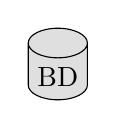
\begin{tikzpicture}[shape aspect=.5]
				\tikzset{every node/.style={cylinder, shape border rotate=90, draw,fill=gray!25}}
			\node  at (1.5,0) {BD};
			\end{tikzpicture}}}{}   
			
			% Display the calls between nodes	
			\begin{sdblock}{Ballot contract registration}{}

				\postlevel
				\begin{call}
					{EVR}{\shortstack{Send ballot creation details.\\{[}ballotName, ballotOptions, ballotEndDate{]} }}
					{OBR}{Response {[}Ok{]}}
					
					\begin{call}
						{OBR}{\shortstack{Create login credentials for voter\\{[}voterID, nonce{]} } }
						{B}{Response {[}ballotAddress{]}}
						\postlevel
					\end{call}
					
					\postlevel
					\postlevel
					\begin{call}
						{OBR}{\shortstack{Save ballot details to databse\\{[}ballotName, ballotAddress{]} } }
						{OBR}{Response {[}Ok{]}}
						\postlevel
					\end{call}
				\end{call}
  			\end{sdblock}
  		\end{sequencediagram}
  	
  	}%
	\caption{Registering a new ballot in the blockchain.}
\end{figure}

The \textit{Online Ballot Regulator} does two things, first registering the ballot contract into the Blockchain with the information received from the remote call. This is funded (and therefore deployed) by the \textit{Ballot Regulators} private key and corresponding Ethereum address which, due to the programming of the ballot contract, means that the ballot regulator has exclusive rights to modify the contract. Deploying the contract happens in three stages in the \href{https://github.com/Mattie432/Blockchain-Voting-System/blob/master/Programming/4_OnlineBallotRegulator/ethereum/ethereum.py}{ethereum/ethereum.py} class of the \textit{Ballot Regulator}. First, the contract `template' is deployed to the Blockchain via the Ethereum software run on the server. This is done by sending the compiled contracts bytecode in an Ethereum transaction along with the contract parameters needed to initially setup the contract (the ballot name \& ballot end time). Once the contract is deployed and confirmed into the blockchain we can access the contract at a specific address which we will use from here on out to interact with the contract (e.g. \href{https://etherscan.io/address/0x127c73af1f9e0eff8226db6bdf04310fdee674f6}{0x127c73af1f9e0eff8226db6bdf04310fdee674f6}).

Next we send another transaction for each ballot option, calling an internal method of the contract, to add each of the options to the deployed contract (you can see examples as the 2nd and 3rd transactions in the above link). These options are then immutably added as choices of the ballot.

The final transaction to the contract is to the internal `finalize()' method. After which, no more ballot options can be added and any registered voters are able to cast their votes.

Once the ballot has been deployed to the blockchain the \textit{Ballot Regulator} confirms its validity and then stores internally the ballots name \& Blockchain address. This allows us to query the \textit{Ballot Regulator} later to obtain the correct address for a specific ballot.


\cleardoublepage
\subsubsection{Registering voters in our system}
Once we have a voter who wishes to register, and is eligible to voter in a specific ballot (or set of ballots) we need to add this user to our system so they can log in \& vote.

\begin{figure}[h]
	\noindent
  	\makebox[\textwidth]{

		\begin{sequencediagram}
			
			% External; Voter registration
    		\newthread{EVR}{\shortstack{External Voter \\Registration}}
			
			%Voter
   			\newinst[2]{V}{\shortstack{Voter \\ \\ 
\begin{tikzpicture}
				%\node [fill=gray!20,draw=black,thick ,align=center] {Procesos};
				\draw (0,0) -- (0,0.5); 			%body
    			\draw (-0.25, 0.25) -- (0.25,0.25); 	% arms
    			\draw (0,0) -- (0.25,-0.25); 		% right leg
			    \draw (0,0) -- (-0.25,-0.25);		%left leg
			    \draw (0,0.7) circle(.2); 	% head
			\end{tikzpicture}}}{}

			%Application server
			\newinst[2]{AS}{\shortstack{Application\\Server}}			
			
			%Online account verifier
			%\newinst[1]{OAV}{\shortstack{Online Account\\Verifier}}
			
			%Online ballot regulator
			\newinst[2]{OBR}{\shortstack{Online Ballot\\Regulator}}
			
			% Blockchain
    		%\newinst[1]{B}{\shortstack{Blockchain \\\begin{tikzpicture}[shape aspect=.5]
			%	\tikzset{every node/.style={cylinder, shape border rotate=90, draw,fill=gray!25}}
			%\node  at (1.5,0) {BD};
			%\end{tikzpicture}}}{}   
			
			% Display the calls between nodes	
			\begin{sdblock}{Pre-election registration}{}

				\postlevel
				\postlevel
				\begin{call}
					{V}{\shortstack{Voter registers\\with external\\registrar}}
					{EVR}{\shortstack{Send voter login\\ credentials\\{[}voterID, nonce{]} }}
					
			 	\postlevel
				\begin{call}
					{EVR}{\shortstack{Create login credentials for voter } }
					{AS}{Returned account details{[}voterID, nonce{]}}
				\end{call}
				
				\postlevel
				\postlevel
				\begin{call}
					{EVR}{\shortstack{Inform the verifier of this voter \& their associated ballot(s)\\{[}voterID, ballotID{]} }}
					{OBR}{Ok}
				\end{call}
				
				\postlevel
				\postlevel
				\end{call}
  			\end{sdblock}
  		\end{sequencediagram}
  	
  	}%
	\caption{Sequence diagram showing order of calls when a voter is registered with our system.}
\end{figure}

The first step is validating the user requesting to register is eligible to vote. The validation process is out of the scope of this project but you could imagine this being a similar process to current election registration schemes. Therefore our system has no verification built in and allows anyone to sign up for any ballot of their choosing.

Next we request a new user account is created in the \textit{Application Server} for our voter. A network request is sent and handled by the \href{https://github.com/Mattie432/Blockchain-Voting-System/blob/master/Programming/2_ApplicationServer/accounts/remote_user_add.py}{accounts/remote\_user\_add.py} class which generates a new userID \& random secure password which are then passed back to the caller.

We now register the userID for any ballots they are eligible for. This is done in another network call to the \textit{Online Ballot Regulator} and is handled in the \href{https://github.com/Mattie432/Blockchain-Voting-System/blob/master/Programming/4_OnlineBallotRegulator/onlineballotregulator/network_request.py}{onlineballotregulator/network\_request.py} class. A database entry is created linking the userID to a ballotID  which is used later to verify which ballots a logged in user is eligible for.

Finally the login credentials are sent securely to the user using an applicable method. For a more traditional registration system, this could be sent in the post similar to how you receive a credit card \& pin number (separate letters). It would be possible to encode this information into a QR code format so that the end user need simply scan their received credentials to first log into the system. If the voter validation process was online based, i.e. allowing users to upload their identity documents for automatic processing, we could respond with the users login details almost instantly just like signing up to any secure website (the risks here are reduced as the user is required to change their password on first login anyway).

\begin{figure}[h]
	\noindent
	\vspace{-0.5cm}
  	\makebox[\textwidth]{\includegraphics[width=0.62\paperwidth]{external_voter_registration_register_new_user}}%
	\caption{Screenshot of the web interface to the \textit{External Voter Registration} showing the previously created ballots at the top \& the ability to register a new user (to a set of ballots) at the bottom.}
\end{figure}


\cleardoublepage
\subsection{During the Election}
\subsubsection{First login}
\subsubsection{Online Registration}
\subsubsection{Voting}

\cleardoublepage
\subsection{Post Election results}
\subsubsection{Retrieving results}
anyone can, openly verifiable


%\printbibliography

\end{document}
	
	\cleardoublepage
	
\blankpage

	\documentclass{article}
\usepackage{graphicx}
\usepackage{standalone}
\usepackage{multicol}
\usepackage[parfill]{parskip}

% Used for sequence diagram
\usepackage{pgf-umlsd}
\usepackage{tikz}
\usetikzlibrary{shapes,arrows}

%used for subsubsubsections
\setcounter{tocdepth}{5}
\setcounter{secnumdepth}{5}

\usepackage{changepage}   % for the adjustwidth environment

% for currency
\usepackage{siunitx}

% syntax highlighting
\usepackage{listings} 
\usepackage{color}
\definecolor{lightgray}{rgb}{.9,.9,.9}
\definecolor{darkgray}{rgb}{.4,.4,.4}
\definecolor{purple}{rgb}{0.65, 0.12, 0.82}
\definecolor{codegreen}{rgb}{0,0.6,0}
\definecolor{codegray}{rgb}{0.5,0.5,0.5}
\definecolor{codepurple}{rgb}{0.58,0,0.82}
\definecolor{backcolour}{rgb}{0.95,0.95,0.92}
\lstdefinelanguage{JavaScript}{
  keywords={typeof, new, true, false, catch, function, return, null, catch, switch, var, if, in, while, do, else, case, break},
  keywordstyle=\color{blue}\bfseries,
  ndkeywords={class, export, boolean, throw, implements, import, this},
  ndkeywordstyle=\color{darkgray}\bfseries,
  identifierstyle=\color{black},
  sensitive=false,
  comment=[l]{//},
  morecomment=[s]{/*}{*/},
  commentstyle=\color{purple}\ttfamily,
  stringstyle=\color{red}\ttfamily,
  morestring=[b]',
  morestring=[b]"
}

\lstset{
   language=JavaScript,
   backgroundcolor=\color{lightgray},
   extendedchars=true,
   basicstyle=\footnotesize\ttfamily,
   showstringspaces=false,
   showspaces=false,
   numbers=left,
   numberstyle=\footnotesize,
   numbersep=9pt,
   tabsize=2,
   breaklines=true,
   showtabs=false,
   captionpos=b
}

% Hyperlinks
\usepackage[colorlinks,allcolors=blue]{hyperref}
\usepackage[normalem]{ulem}
\usepackage{xcolor}
\makeatletter
\begingroup
  \catcode`\$=6 %
  \catcode`\#=12 %
  \gdef\href@split$1#$2#$3\\$4{%
    \hyper@@link{$1}{$2}{\uline{$4}}% or \underline
    \endgroup
  }%
\endgroup

%Used for bibliography
\usepackage[british]{babel}
\usepackage[%
  autolang=other,
  backend=bibtex      % biber or bibtex
%,style=authoryear    % Alphabeticalsch
 ,style=numeric-comp  % numerical-compressed
 ,sorting=none        % no sorting
 ,sortcites=true      % some other example options ...
 ,block=none
 ,indexing=false
 ,citereset=none
 ,isbn=true
 ,url=true
 ,doi=true            % prints doi
 ,natbib=true         % if you need natbib functions
]{biblatex}
\addbibresource{../Bibliography/Bibliography}

\begin{document}
    \section{Project Analysis}
    \subsection{Overview}
	With this project I intended to create a proof-of-concept system for an `end-to-end' verifiable voting platform. While previous sections discussed the rationale, design and implementation, I now intend to analyse the projects success and viability.

	The project succeeds in presenting the protocol for an `end-to-end verifiable system' through use of Blockchain technology. The system is \textit{individually verifiable}, voters can check that their vote was successfully included in the Blockchain and can ensure that their vote was cast as intended (the stored result matches what the voter wanted). It is also \textit{universally verifiable} as anyone, whether they are participating in the election or not, can verify the results of the election \&, due to the systems design, be assured that each voter was only able to vote once per ballot.
	
	The associated costs with deploying a similar system on the scale of a general election look, not only feasible, but substantially less than current means. As this estimate is tied to the traded price of Ethereum we can expect some fluctuations in the actual cost but even with an exponential increase the costs should be less than a traditional election.
	
	Finally the scalability of the system, while not currently being able to process the vast number of transactions a general election would generate, does look like it will acquire the necessary throughput in the near future.
	
    \clearpage
    \subsection{Financial Feasibility}
	Using the Ethereum network as our distributed database comes at a cost. Obviously this requires computing power as the network ensures the integrity of the Blockchain along with processing new transactions into it and these computers need to be incentivized to continue providing this service.
	
	Is it important to understand what actually costs money in the system. You only pay for remote computation or data entry transactions so, in this system the only places we have an external cost are during poll creation and voting. Whenever we create a poll or a user votes we have to send Ether to the Ethereum network that collectively verifies your vote/poll and inserts it into the Blockchain. These are the two areas I have chosen to analyse and both cost money because we are writing data to the Blockchain.
	
	Each transaction has a fixed cost of gas which depends on several factors, such as the amount of computational steps it requires, this number cannot be adjusted as it depends on the transaction code being executed. Each transaction can also set a `gas limit' and a `gas price'. The `gas limit' is used to specify the upper bound of gas you are willing to pay for a transaction (unused gas is returned to the sender anyway) but is essentially used to ensure `buggy code' does not deplete your Ethereum account balance \citep{57_introduction_ethereum_frontier_guide_2017}. The gas cost of the transaction will be bought by the ether you have in your account at a price you specified with `gas price' Higher prices for each unit of gas means miners are more likely to run your contract or that you may overpay. 
	
	\subsubsection{Ballot Deployment}
	Creating a new ballot requires three things (as discussed in \hyperref[sec:CreatingANewBallotContract]{Creating A New Ballot Contract \ref*{sec:CreatingANewBallotContract}}) deploying the contract, adding the ballot options and finalizing the contract. More specifically, we are storing the following information into the Blockchain:
	\begin{itemize}
		\item \textbf{owner} - The address (20 bytes) of the ballot creator.
		\item \textbf{optionsFinalized} - Boolean value of whether the poll is set up.
		\item \textbf{ballotName} - Arbitrary length UTF-8 ballot name.
		\item \textbf{registeredVoterCount} - Integer count of registered voter addresses.
		\item \textbf{ballotEndTime} - Integer value of seconds since epoch.
		\item \textbf{votingOptions} - Dynamically sized array of the `VotingOption' structure (this structure contains a string name and integer vote count).
	\end{itemize}
	
	As you can see we do quite a lot in a varying number of transactions (varying because we add each option in a separate transaction and we can have an unlimited number of options). I calculated the costs associated with all of the ballots I publicly deployed over the course of my testing (\href{https://docs.google.com/spreadsheets/d/1dyLkpD-rdH4eHFEsdPrLEXX45YHl9XLGppbYgYYsTOo/edit?usp=sharing}{spreadsheet available here}) and found that while the average cost of fully deploying a contract (including adding multiple ballot options and finalizing) is around \pounds0.96 the individual cost vary considerably depending on the data being added (minimum cost was \pounds0.79 for a 2 option ballot and maximum was \pounds1.17 for a 6 option ballot). Changes in cost here seem to depend most on the number of options being added and the length of the string in each of those options.
	
\begin{figure}[h]
	\noindent  	
  	\makebox[\textwidth]{
  	    \begin{tabular}{ | l | S |}
    		\hline
    		\textbf{Description} & \textbf{Average Cost ({\pounds})}\\ \hline 		
			
			Average cost of the initial deployment. & 0.71 \\ \hline
			
			Average cost of adding a ballot option. & 0.05 \\ \hline
			
			Average cost of finalizing the contract & 0.02 \\ \hline
			
			Average cost to fully deploy a ballot & \\ (initial deployment, option addition and finalization). & 0.96 \\ \hline
    		   		
    		
    	\end{tabular}
  	}%
	\caption{Average cost of deployment actions (prices calculated April 2017).}
\end{figure}

	\subsubsection{Adding voters}
	The next cost incurred by the system is during the addition of voter addresses to the deployed ballot contract. Due to the fixed length of voter addresses (20 bytes) this type of transaction will always have the same amount of data being added to the blockchain; therefore we will always use the same amount of gas, 49100, for each transaction.

	\begin{figure}[h]
		\noindent
  		\makebox[\textwidth]{\includegraphics[width=1.07\textwidth]{cost_voter_addition}}%
		\vspace*{-0.3cm}
		\caption{Cost of registering a voter address over time tracking the inflation of Ethereum.}
	\end{figure}	
	\clearpage
	
	Therefore the only cost variable here is the `Gas Price' (the Ether price we buy a unit of gas for) which is tracked to the traded price of Ethereum. This means that the price we pay for adding a voter to a ballot contract will fluctuate over time with the price of Ethereum.

	Currently (April 2017) the price of Ethereum is around \pounds35.26 resulting in a price per address registered of \pounds0.04. Data released under the public information act \citep{69_statistics_from_2010_election} states that, during the 2010 UK General Election, there were 45,597,461 registered voters on the UK Parliamentary Register. To register this many people on our system at a cost of \pounds0.04 per voter, would equate to \pounds1,823,898. Even if we assume that the increased rate of inflation of Ethereum continues, an estimate of more than double the current Ethereum costs (\pounds £0.10 per voter) would cost around \pounds5 million. For perspective the cost to print, dispatch and return the postal votes for the 2010 election were around \pounds10.6 million \citep{70_what_price_democracy_counting_the_cost_of_uk_elections}.
	
	\subsubsection{Voting}
	The final area of cost relating the the ballot contracts is that of voting. And additional consideration here is allowing user to change their vote, as the cost incurred each time a vote is cast but more computation needs to be done on subsequent casts (due to the removal of the previous vote allocation).
	
	
	\begin{figure}[h]
	\noindent  	
  	\makebox[\textwidth]{
  	    \begin{tabular}{ | l | l |}
    		\hline
    		\textbf{Description} & \textbf{Average Cost ({\pounds})}\\ \hline 		
			
			Average cost of the initial vote. & 0.025 \\ \hline
			
			Average cost of re-voting. & 0.045 \\ \hline
    		   		
    	\end{tabular}
  	}%
	\caption{Average cost of per user voting and re-voting (prices calculated April 2017).}
	\end{figure}

	As you can see from the average costs table, the cost of re-voting is a little under half of the cost of the initial vote meaning it's not prohibitively expensive in relation to the original voting cost.
	
	If we calculate these prices with in relation to the registered number of voters in the 2010 election (45,597,461) \citep{69_statistics_from_2010_election} we find that cost for everyone to vote once would be around \pounds1,139,936.53 and the cost of everyone submitting a subsequent vote being \pounds2,051,885.75. 
	
	To represent this information in another form, these costs would mean (prices taken April 2017) that 1000 initial votes would cost the system \pounds25, 1000 re-votes would cost \pounds45, an individual casting their vote then changing their mind twice would cost \pounds0.115 and 1000 people doing so would cost \pounds115.

	\subsubsection{Cost Comparison}

	While initially looking at the above costs on a per-voter basis you might think that these prices are too high to be competitive with traditional voting techniques, however when broken down, we see a potentially different picture. As you might suspect, holding elections today is expensive and slow. The system is still based off of physical booths, paper ballots and requires humans to count the ballots (in some cases there are machines counting the ballots, but this is often more expensive than humans on a per voter cost basis \citep{71_arthur_2017}.)

	To compare this Ethereum-based voting system to the current voting system I'm using data from the 2010 UK General Election where the vote turnout was at 65.1\%. Therefore, out of 45,597,461 registered voters 29,991,471 actually voted \citep{72_voter_turnout_at_uk_general_elections}. The estimated the cost of this general election was \pounds113,255,271 \citep{70_what_price_democracy_counting_the_cost_of_uk_elections}  of which \pounds28,655,271 was the cost of distributing candidates mailings and a further \pounds84.6 million was for the conduct of the poll. This means that, on average, it cost about \pounds3.77 to register and count a vote but if we were to only take the costs for conducting the poll (\pounds84.6 million), it would cost \pounds2.82 to cast a single vote.

	Therefore we can compare the cost of using our Ethereum based voting system to the traditional system for this election. Remember that the average cost of the initial vote in our system was \pounds0.025, which means that if all of the voters were to use our system it would cost a total of \pounds749,786.75 to process these votes into the blockchain. Whilst this number might not be completely correct as we are presuming a lot (such as the price of Ethereum being the same, the fact that all of these votes would be using our system, and not counting the costs of running the backend of this system), it does put into perspective the potential cost savings when compared to traditional means.
	
	To compare, the traditional voting system would be around 3800\% (38x) more expensive than a blockchain voting system in this scenario. This breaks down to the cost of casting each vote being \pounds2.82 in the traditional system to \pounds0.025 in our system.
	
	With this margin of cost savings we could afford to let every voter re-vote up to 21 times and still cost less that the traditional system. This is likely an underestimate of the actual number as its unlikely everyone would choose to re-vote.
	
	\clearpage
	\subsubsection{Cost minimization strategy}
	In Ethereum, each instruction in the Turing complete scripting language has an associated cost when executed, along with additional costs for writes to the Blockchain. These costs are counted in gas and the user specifies the price per gas unit that they are willing to pay. Permanent storage to the Blockchain dominate transaction costs, it currently costs 3 gas to perform an addition but 20,000 gas to store a single 256-bit integer.
	
	As each operation consumes a calculable amount of gas we can aim to minimize the gas used through careful contract design. Simplifying the contract as much as possible is a good way to start but we could also look into more subtle ways to reduce costs such as choosing storing the voters ballot choice as an index (integer) rather than a string.
	
	We can also look at the contract at a higher level, for example the contract I have written for this system uses multiple transactions to setup the contract (one for the initial deployment, one for each ballot option and a one to finalize). I was unable (at the time of writing the contract but future language updates should fix this) to send an arbitrary number of strings in the constructor of the contract due to current limitations of the EVM. Therefore I settled on using multiple transactions to maintain this functionality rather than compromise the contracts usability. Once the EVM has been updated and is able to handle this sort of information, we could compress this into one singular call to deploy the contract with all of the ballot options minimizing the cost of setting up a ballot.
	
	There is also the potential for analysis of the optimal gas price to set for each transaction. As miners can choose which transactions to accept based on the amount of computation and the gas price of the transaction, we could work out the most effective price to use at a given moment in time to minimize both the cost to us and the transaction confirmation time. Though the savings per transaction would likely be minimal, when scaled to the numbers involved in a general election the compounded savings could be of reasonable note.
	
		
	\clearpage
	\subsection{Scalability}
	Throughout this paper I have been working on the assumption that the Ethereum network would be able to handle the amount of transaction volume a general election would bring. 
	
	At the current gas limit of 4,019,884, at the cost of 42182 gas per initial vote, we could only register some 95 votes every 12 seconds. That is about 684,000 in a day. Therefore, holding the General Elections on the Ethereum Blockchain would take around 43 days to complete. This is of course not acceptable and therefore can say that, at the current time, the Ethereum Network does not have the capacity to scale to this level. This problem is more general than the Ethereum network and is currently inherent to blockchain technologies, the same scalability problems currently exist across all other protocols.
	
	However, Ethereum has some scaling properties already built in. While there is a `Block Gas Limit' governing how many transactions can be confirmed in a single block, this limit (unlike other protocols such as Bitcoin) is not fixed and does in fact have the ability to adjust after every confirmed transaction. Miners can choose to change the gas limit $\pm\frac{1}{1024}$ depending on the networks gas consumption at a given time. Block gas limits scale indefinitely \citep{73_wood_2017} so under excessive demand we can expect to see more transactions per block.
	
	A more recent and promising development was that Vitalik Buterin, founder of Ethereum, has laid out an ambitious roadmap with ``unlimited'' transaction scalability within two years \citep{74_ethereum_announces_unlimited_scalability_roadmap}. The changes have been outlines in a yellow-paper \citep{73_wood_2017} and introduce the idea of `sharding' to the Ethereum network which would ultimately mean that not every node needs to process every transaction. 
	
	\textit{``The long term goal for Ethereum 2.0 and 3.0 is for the protocol to quite literally be able to maintain a blockchain capable of processing VISA-scale transaction levels, or even several orders of magnitude higher, using a network consisting of nothing but a sufficiently large set of users running nodes on consumer laptops.''} - Vitalik Buterin, 2016 \citep{74_ethereum_announces_unlimited_scalability_roadmap}.
	
	The changes outlined in this paper would allow throughputs of around 10000+ tx/sec \citep{75_eip_105} which would more than cover the needs of our system. Currently, Ethereum is the only protocol who is actively working towards sharding as a solution to the scalability problems which gives further validity to the choice of using it for this system.
	
	\clearpage
	\subsection{Privacy}
	Voter privacy (i.e. the inability to link a voter to a vote) is the most important property of a voting system because once it is compromised, coercion and collusion cannot be avoided and therefore no other requirement can be assured \citep{48_safevote_2001}. 
	
	The design of the system ensures that, with the exception of the securely stored private key of each voter, there is no information retained which could link a user account (and the individual behind it) to an Ethereum address. Unfortunately, there is still a degree of trust which must be instilled in the central authority that they are running this system as described and maintaining this secrecy which many users may be unwilling to do. While open sourcing the codebase could alleviate some this there will always be some parts of the system behind closed doors though how to gain the public's trust in such a system is beyond the scope of this paper.
	
	\subsubsection{Voter Obfuscation}
	Due to the public nature of the votes being cast in a Blockchain, we need to be aware of the possibility for a voter to inadvertently leave a trail which could be followed and directly identify them. The main concerns here would be based around some form of statistical analysis being able to discern potentially identifying traits of a voters Ethereum address. 
	
	\paragraph{New voting address per ballot}
	\hfill \break \break
	One possible way for an address to become less anonymized would be if it was used for multiple ballots. For example, if you could see that an address voted in a particular regional ballot and that they were the only ones to vote for a particular candidate while being externally vocal about their opinions on this particular ballot. You could determine who that individual was and then, because they used the same address for other ballots, see other voting choices.
	
	The system actually takes steps to eliminate this possibility. We generate a new, unique voting address for each ballot the voter registered to participate in. As address creation is very cheap and the address space is incredibly large, it makes sense to generate a new address each time while incurring almost no additional overhead. This means that there is no chance to link addresses across ballots, as each address is only used for a single ballot.
	
	\clearpage
	\paragraph{Transaction timings}
	\hfill \break \break
	Another possibility for statistical analysis could be found in the timing of transactions being submitted. For example while testing the system, as there was very few users actively voting concurrently, it was easy to determine which transactions were mine as they were the only ones being sent. Applying this more generally, maybe an ISP could see the times you accessed the voting web interface and if there were sufficiently few transactions during that time we could trivially link your voting choice to you.
	
	While this problem is significantly reduced when the system is used by a larger number of people, we could also employ tactics such as modulating the `gas price' of the transaction to increase the amount of time between it being submitted and confirmed. Whilst its desirable to be able to see your vote as `confirmed' almost instantly, it is not strictly necessary. As long as you can see that is has been included in the pool of unconfirmed transactions you can assume with relative certainty that is will be accepted at some point in the future.
    
    \subsubsection{Voter coercion}
    Though illegal the removal the guaranteed secrecy of a polling booth does open the possibility for increased levels of voter coercion when using this system.    
    
	\paragraph{Vote buying}
	\hfill \break \break
	The transparency of this system undermines the basis of vote buying. To ensure that the purchased votes were not merely promised, the vote buyer would be compelled to collect vote receipts and to record the identities of the sellers. He would also have to ask the vote seller to forgo payment until after the election results had been finalized (as a voter can change their vote up to the election deadline). Therefore as the sellers would have no means of enforcing the completion of the transaction the low level of trust between buyer and seller would make this form of vote buying unlikely.

	Even if a valid voting receipt, in the form of a transaction hash, was presented for payment after the election it would similarly be of no value. Since all votes are publicly broadcast, anyone could submit any transaction hash that was cast in favour of a particular candidate as this receipt is proof that a ballot has been cast, but gives no indication who cast it, a buyer is unlikely to pay in this scenario.

	\clearpage
	\paragraph{Forced voting}
	\hfill \break \break
	One concern unique to this way of voting, is the guaranteed return of a receipt for each vote cast in the form of the transaction hash. The returning of this hash is inescapable, as its a core part of the blockchain functionality and provides the only way for a voter to validate that their transaction was included into the blockchain. 
	
	The problems of community pressure, are mitigated by the fact that (as mentioned in the previous section), a voter can provide any transaction hash as a receipt and it is not individually identifiable. Therefore requesting a receipt to prove the way an individual voted does not work.
	
	A more realistic problem however is, due to the lack of a polling booth, individuals can be forcibly made to vote in a particular way. I was unable to think of a direct way to combat this, however I propose a method for a voter to discreetly mark these forced ballots as such and for them to not be counted in the ballot tally.
	
	As the user is required to enter a password to unlock the Ethereum account before a transaction can be authorized, I would introduce the idea of a `panic password' at this stage. Panic passwords gained traction as a safety measure for ATM transactions. It is a special password or set of actions which the user can trigger to alert the server that the user is under duress. In this system it could be that the user enters their password in reverse to trigger the panic status.
	
	Once this occurs, the system continues as usual processing the transaction and providing a receipt except with the addition of a flag as part of the transaction which ultimately invalidates this vote in the contract. This would mean the person forcing the vote would be none the wiser as externally it would appear the same as a regular vote.	
	
	\clearpage
	\subsection{System security}
	\subsubsection{The Ethereum Network}
	 With the scope of this project aiming to design a secure voting system, possibly usable in a general election, it's essential to confirm the level of security and to understand the risks involved with the Etherum network.

Ethereum while not branded as a cryptocurrency, is often traded on cryptocurrency exchanges and as the name suggests, cryptography is a central part of the protocol. Ethereum makes use of the KECCAK-256 cryptographic hashing function (essentially SHA-3 before standardization).

Signatures in Ethereum are performed exactly the same as in conventional public-key cryptography. We can verify that Alice is the owner of a transaction because she has signed it with her private key, which can then be verified with her public key. Ethereum uses the ECDSA elliptic curve for generating the key pairs which appears to have been chosen for possible speed optimizations in the future \citep{41_yang_2011}. Attacks here could involve breaking the underlying elliptic curve cryptography either by solving the discrete logarithm problem (which could be possible with quantum computers, but there is currently no efficient non-quantum algorithm), or by finding vulnerabilities in the specific curve chosen.

As with most public-key cryptography, Ethereum does not sign the entirety of the transaction as this would be too expensive. Instead, it signs a hash which can then be checked against the transaction to verify its integrity. If we could break the hash function, it could be possible to generate a secondary input transaction to hash to the same value as an original. This could then be used to perform a signature replay attack to forge a transaction.

The likelihood of either of these two scenarios being immediate threats is however, relatively low. Ethereum uses industry standard technology and a breach in any of the underlying cryptography would undermine a large proportion of the security we enjoy on the internet. 

Despite the underlying cryptography being secure, there are still a number of possible attacks which could be utilised against the network. While a dishonest miner cannot generate Ether (illegitimately), steal Ether from an account or make payments on your behalf (pretend to be you), they could delay or refuse the relaying of valid transactions to other nodes, attempt to create blocks which exclude specific transactions of their choosing or attempt to create a longer blockchain that would render previously accepted blocks invalid \citep{22_brave_new_coin_2016}. However all of the above require the attacker to have sufficient block creation power, effectively a 51\% attack on the network. When an individual or group owns more than half of the network they could produce enough ``computational work'' to convince others that their blockchain is the best choice \citep{41_yang_2011}.

This became a real threat on the Bitcoin network in January of 2014 as the mining group \textit{Gash.io} started to approach 50\% of the mining power of the entire network. At one point the group had collectively solved 42\% of the blocks in a 24 hour period \citep{42_liu_2014}. The situation was resolved without incident, due to miners leaving \textit{Gash.io} for smaller pools, as well as the pool’s own decision to stop accepting new miners \citep{41_yang_2011}.
	
	\subsubsection{Voter key management}
	As with the various types of Bitcoin and Ethereum wallet software available there is always a trade-off between user managing their own keys and online services doing it for them. Storing private keys on behalf of users is a very dangerous thing to do, especially if we are talking about a general election which would be of great interest to hackers. However, the truth of the matter is that the vast majority of people lack the skills needed to properly protect such information by themselves.
	
	For this reason the system should be designed to securely store the encrypted private keys of each user in its internal database. This encryption should be of sufficient strength, AES-256, and while being password based we should enforce a different password than the one a voter uses to log into the system (as this could present a risk that if the server becomes compromised an attacker would trivially be able to affect the votes in the blockchain).

	This is a difficult problem to solve, companies such as LastPass get around this by only ever seeing an encrypted version of your private data (as encryption and decryption happen client side). This approach opens the user to the possibility of being compromised and also would also require sending the private key over the wire to authenticate a transaction (though this concern may be mitigated with secured connections).
		
	A potential alternative could be to enforce the user to print out their private key (similarly to a paper wallet) in the form of a QR code. This could then be scanned in when necessary to unlock the account and authorize a transaction. Although this approach might reduce the chances of keys on a voters computer being compromised, it still places the security of the voters ballot in the voters hands.

	\subsubsection{Loss of Ether}
	\label{sub:LossOfEther}
	Because we fund each users account with enough Ether to submit a transaction vote, there is potential for a large scale loss of Ether either to occur. This could be through over supplying ether to accounts or by users attempting to game the system. 
	
	For the proof-of-concept, the system currently supplied 0.005 Ether to each registered account so that they may perform around 4 to 5 transactions. This is obviously not the best way to implement this when scaling to the level of a general election as, say for example the user only votes once then the remaining Ether goes unspent at cost to the system. It also incentives people to attempt to game the system as they see this as free money (albeit a very small denomination) which they may attempt to transfer into a private account.
	
	As a potential future improvement I suggest a system where we always fund the voter address with enough Ether to conduct one additional vote. This amount should be calculated based on predicted gas and Ether prices and should include a degree of leniency in favour of over funding. When a user submits a vote, their account is automatically topped up the to required level to be able to submit another one. In this way, we eliminate the over funding problem for those accounts who were never going to re-cast their votes while still allowing those who do wish to, unlimited voting opportunity.
	
	This system however could be easily exploited due to the slight over funding to compensate for price fluctuations. A user could re-vote multiple times to accumulate an excess of Ether which could then be siphoned off. To compensate for this, some form or rate-limiting could be employed (maybe 3 re-votes per hour) along with a check of whether the voters account has enough to cast another vote before funding it again.
	
	\subsubsection{Individual computer security}
	Moving an election of any type away from the security of a polling booth and on to individuals computers, phones and laptops presents many security issues. The potential for an attacker to compromise an uneducated user's computer is relatively high and an event such as a general election would undoubtedly produce more attempts to do so.	As voting options are conducted through a web interface, the possibility of XSS attacks or attempts to miss-represent one voting option as another must be considered.
	
	Therefore alongside strong secure design, as a minimum voters should be educated on basic computer security that would allow them to increase the difficulty for an attacker to compromise an individual voter.	
	
	We could also enforce certain security requirements on the user, such as running an up-to-date OS version or requiring certain security software to be installed and active. But this must not raise the barrier to entry so much that we alienate a group of the voting populous (for example the elderly might not be able to easily conform to these requirements).
	
	\clearpage
	\subsubsection{Direct contract interaction}
	For the most security conscious we could allow direct contract interaction from an individual. This would likely only be undertaken by a handful of people but it would still require them to use some parts of the system to submit an address which they wish to use and have it added to the ballot contract in the blockchain. Ultimately though this would still be heavily reliant on system interaction which would be what people wishing to conduct this interaction will be most critical of.
	
	It may be possible to move more of the inner workings of the system on to the blockchain its self. Although some form of verification will still need to happen, users could interact with a smart contract in order to have their private addresses added to the list of allowed voters. Having more of the system become transparent would be beneficial not only to these more sceptical individuals but increase trust in the system as a whole.
    
\clearpage
\subsection{Improvements}
Reflecting upon the project, there are a number of design decisions which I would consider doing differently next time.

\subsubsection{Implementation}
Firstly, I would run Geth (the Ethereum software) in its own Docker container. Currently it is being run inside the ``Online Ballot Regulator'' and could be easily extracted for a more modular system. Running it in its own container would further segregate the various sections of the application providing increased security and decouple the files of the ``Ballot Regulator'' from any files generated by Geth.

I would also serve the web application over Apache (or a similarly established software). Currently the system is running off of Django's built in webserver which, while fine for development, it is a stripped-down, very basic, single-threaded server for the purposes of development and has not gone through the required security audits or performance tests for production deployment. Transferring the server over to Apache would be trivial to setup with the WSGI interface.

\subsubsection{Protocol}
There is a glaring omission in the design of the ballot contract, the opportunity for voters to practice their right to suffrage. Currently the ballot contract template does not add any option for a `non-vote' which should be included to maintain voter rights.

This could be easily implemented with minimal change to the solidity contract. We could add an extra ballot option titled `non-vote' or similar during the finalization state of ballot creation meaning it would be automatically applied to all ballots.

I would also re-implement the way voter accounts receive funding to allow them to vote (also discussed in the \hyperref[sub:LossOfEther]{Loss of Ether \ref*{sub:LossOfEther}} section). Essentially I would change it to a top-up system where more Ether is allocated to your account when you vote rather than giving it all to you in one go. This reduces unnecessary allocation of funds to voters who will only use their initial vote and reduces the likelihood of an individual attempting to game the system.


\end{document}
	
	\cleardoublepage
	
\blankpage

	\documentclass{article}
\usepackage{graphicx}
\usepackage{standalone}
\usepackage{multicol}
\usepackage[parfill]{parskip}

% Used for sequence diagram
\usepackage{pgf-umlsd}
\usepackage{tikz}
\usetikzlibrary{shapes,arrows}

%used for subsubsubsections
\setcounter{tocdepth}{5}
\setcounter{secnumdepth}{5}

\usepackage{changepage}   % for the adjustwidth environment

% syntax highlighting
\usepackage{listings} 
\usepackage{color}
\definecolor{lightgray}{rgb}{.9,.9,.9}
\definecolor{darkgray}{rgb}{.4,.4,.4}
\definecolor{purple}{rgb}{0.65, 0.12, 0.82}
\definecolor{codegreen}{rgb}{0,0.6,0}
\definecolor{codegray}{rgb}{0.5,0.5,0.5}
\definecolor{codepurple}{rgb}{0.58,0,0.82}
\definecolor{backcolour}{rgb}{0.95,0.95,0.92}
\lstdefinelanguage{JavaScript}{
  keywords={typeof, new, true, false, catch, function, return, null, catch, switch, var, if, in, while, do, else, case, break},
  keywordstyle=\color{blue}\bfseries,
  ndkeywords={class, export, boolean, throw, implements, import, this},
  ndkeywordstyle=\color{darkgray}\bfseries,
  identifierstyle=\color{black},
  sensitive=false,
  comment=[l]{//},
  morecomment=[s]{/*}{*/},
  commentstyle=\color{purple}\ttfamily,
  stringstyle=\color{red}\ttfamily,
  morestring=[b]',
  morestring=[b]"
}

\lstset{
   language=JavaScript,
   backgroundcolor=\color{lightgray},
   extendedchars=true,
   basicstyle=\footnotesize\ttfamily,
   showstringspaces=false,
   showspaces=false,
   numbers=left,
   numberstyle=\footnotesize,
   numbersep=9pt,
   tabsize=2,
   breaklines=true,
   showtabs=false,
   captionpos=b
}

% Hyperlinks
\usepackage[colorlinks,allcolors=blue]{hyperref}
\usepackage[normalem]{ulem}
\usepackage{xcolor}
\makeatletter
\begingroup
  \catcode`\$=6 %
  \catcode`\#=12 %
  \gdef\href@split$1#$2#$3\\$4{%
    \hyper@@link{$1}{$2}{\uline{$4}}% or \underline
    \endgroup
  }%
\endgroup
%Used for bibliography
\usepackage[british]{babel}
\usepackage[%
  autolang=other,
  backend=bibtex      % biber or bibtex
%,style=authoryear    % Alphabeticalsch
 ,style=numeric-comp  % numerical-compressed
 ,sorting=none        % no sorting
 ,sortcites=true      % some other example options ...
 ,block=none
 ,indexing=false
 ,citereset=none
 ,isbn=true
 ,url=true
 ,doi=true            % prints doi
 ,natbib=true         % if you need natbib functions
]{biblatex}
\addbibresource{../Bibliography/Bibliography}

\begin{document}
    \section{Conclusion}
	Although this system has been designed and developed with the idea of a national general election in mind, the protocols and ideas involved could be applied to smaller scale ballots which wish to provide transparency in their audit. Although we wish to minimize trust in a central authority, due to the nature of these type of elections (where there needs to be some degree of voter eligibility verification), we cannot fully decentralize this system as we need to only allow those eligible the rights to vote. Despite needing to verify an individual we still need to ensure that their votes are publicly anonymous, especially given the public transactions underpinning the blockchain concept while providing the ability for an individual to verify that their vote was correctly counted.

I do not see this system as a direct ``replace all'' for national election voting. I believe there will still be a need for traditional voting implementations in certain situations; for example, maintaining postal vote for the elderly who may not have the technical capability or equipment for online voting. However I do think that this could be phased in along side traditional voting, eventually replacing the pre-existing e-voting systems and ultimately becoming the main way for the majority of people to choose their government.	

I started this project with the goal of producing an `end-to-end' verifiable voting platform. This project succeeds in presenting the protocol for such a system through use of Blockchain technology.

The system provides \textit{individually verifiability}. When voters submit their vote they receive a transaction hash which they can use to check that their vote was successfully included in the Blockchain. This `cast-as-intender verification' can only be done by the voter, as they are the only one who knows which specific transaction relates to them. While some level of voter education would be necessary for the average voter to desire and be able to check their vote was counted (as the onus of this does still rest with the voter), at worst this is no different from the currently employed systems where uses must trust their vote was submitted and counted correctly while providing benefit to those who engage in it.

The system also provides \textit{universal verifiability} as anyone, whether they are participating in the election or not, can verify the results of the election through querying the ballot contracts. These results hold all of the desirable properties of the Blockchain such as being immutable and instantly globally distributed. Due to the underlying contract design, be assured that each Ethereum address voted at most once per ballot.

The system also manages to protect voter privacy through the use of blinded tokens. This is how the system is able to register an Ethereum address to a ballot contract, without being able to link it to an individual, but they can be assured that it belongs to \textit{some} verified voter. Voter privacy after the election is tied to the voter, as only they know the resulting transaction hash (voting receipt) for each vote cast it is kept private at their discretion.

While the proposed system does not solve all the issues associated with electronic voting, it does provide a valuable alternative to current proprietary electronic systems and has potential use in both governmental and private organizations wishing to conduct transparent ballots.
\end{document}
	
	\cleardoublepage
	
	\section{Appendix}
	\documentclass{article}
\usepackage{graphicx}
\usepackage{standalone}
\usepackage{multicol}
\usepackage[parfill]{parskip}

% Used for sequence diagram
\usepackage{pgf-umlsd}
\usepackage{tikz}
\usetikzlibrary{shapes,arrows}

%used for subsubsubsections
\setcounter{tocdepth}{5}
\setcounter{secnumdepth}{5}

\usepackage{changepage}   % for the adjustwidth environment

% syntax highlighting
\usepackage{listings} 
\usepackage{color}
\definecolor{lightgray}{rgb}{.9,.9,.9}
\definecolor{darkgray}{rgb}{.4,.4,.4}
\definecolor{purple}{rgb}{0.65, 0.12, 0.82}
\definecolor{codegreen}{rgb}{0,0.6,0}
\definecolor{codegray}{rgb}{0.5,0.5,0.5}
\definecolor{codepurple}{rgb}{0.58,0,0.82}
\definecolor{backcolour}{rgb}{0.95,0.95,0.92}
\lstdefinelanguage{JavaScript}{
  keywords={typeof, new, true, false, catch, function, return, null, catch, switch, var, if, in, while, do, else, case, break},
  keywordstyle=\color{blue}\bfseries,
  ndkeywords={class, export, boolean, throw, implements, import, this},
  ndkeywordstyle=\color{darkgray}\bfseries,
  identifierstyle=\color{black},
  sensitive=false,
  comment=[l]{//},
  morecomment=[s]{/*}{*/},
  commentstyle=\color{purple}\ttfamily,
  stringstyle=\color{red}\ttfamily,
  morestring=[b]',
  morestring=[b]"
}

\lstset{
   language=JavaScript,
   backgroundcolor=\color{lightgray},
   extendedchars=true,
   basicstyle=\footnotesize\ttfamily,
   showstringspaces=false,
   showspaces=false,
   numbers=left,
   numberstyle=\footnotesize,
   numbersep=9pt,
   tabsize=2,
   breaklines=true,
   showtabs=false,
   captionpos=b
}

% Hyperlinks
\usepackage[colorlinks,allcolors=blue]{hyperref}
\usepackage[normalem]{ulem}
\usepackage{xcolor}
\makeatletter
\begingroup
  \catcode`\$=6 %
  \catcode`\#=12 %
  \gdef\href@split$1#$2#$3\\$4{%
    \hyper@@link{$1}{$2}{\uline{$4}}% or \underline
    \endgroup
  }%
\endgroup
%Used for bibliography
\usepackage[british]{babel}
\usepackage[%
  autolang=other,
  backend=bibtex      % biber or bibtex
%,style=authoryear    % Alphabeticalsch
 ,style=numeric-comp  % numerical-compressed
 ,sorting=none        % no sorting
 ,sortcites=true      % some other example options ...
 ,block=none
 ,indexing=false
 ,citereset=none
 ,isbn=true
 ,url=true
 ,doi=true            % prints doi
 ,natbib=true         % if you need natbib functions
]{biblatex}
\addbibresource{../Bibliography/Bibliography}

\begin{document}
    \subsection{Source Archive}
Alongside this report is the \href{https://github.com/Mattie432/Blockchain-Voting-System}{accompanying code} for this proof-of-concept system containing everything needed for deployment. Project layout closely follows the \hyperref[sec:SystemDesign]{system design \ref*{sec:SystemDesign}} with the code for each node being contained in its own folder.

\subsubsection{Building}
As I have used Python for each node in my project, I was able to create a \textit{setup} file to create the correct Python environment which can be called using \textit{`pip3 install .'} while in the nodes' root directory.

As I am using docker, building manually is not recommended as there is a lot of environmental setup which must be done. Each nodes' project contains a \textit{Dockerfile} which is used to setup, build and run each application. Each node folder contains a \textit{bin} directory inside which are various executables one of which, \textit{docker\_entrypoint}, is ultimately where we start the systems but the recommended way to start an individual node is to use the \textit{build\_and\_run} executable which combines these steps for ease of use.

\subsubsection{Running}
You can independently start each node through Docker with the \textit{`docker run'} command (conveniently you can run \textit{build\_and\_run} with the parameter \textit{runme}).

This is unnecessary however as Docker provides a tool, Compose, which is used for defining and running multi-container Docker applications. This means I can define a \textit{docker-compose.yml} file in the root directory which will start all of the nodes, with the correct parameters, in the correct order.

This is the recommended way to run this application so calling \textit{`docker-compose up'} while in the root directory should be the most hassle free.

\subsubsection{Notes}

\begin{itemize}

	\item \textbf{Helper Files} - There are a number of helper scripts located in the \textit{HelperScripts} folder which allow for easy interaction with the Docker nodes while running.
	
	\item \textbf{Blockchain download} - As this runs a full Ethereum node and must download the full blockchain before it can push transactions, an initial download of around 20GB will occur on first run.
\end{itemize}
\end{document}

	
	\cleardoublepage
	\subsection{Bibliography}
	\printbibliography[heading=none]
\end{document}
